% =============================================================
% informe_ieee.tex — Criba de Eratóstenes Distribuida con MPI
% Formato IEEE Transactions / Conference
%
% Compilar (dos veces para referencias cruzadas):
%   pdflatex informe_ieee.tex
%   pdflatex informe_ieee.tex
% =============================================================

\documentclass[conference]{IEEEtran}

% Nota: para hifenación en español instalar: sudo dnf install texlive-babel-spanish
% Si el paquete no está disponible, babel sin opción compila sin error.
\usepackage{babel}
\usepackage[utf8]{inputenc}
\usepackage[T1]{fontenc}
\usepackage{graphicx}
\graphicspath{{../resultados/}}
\usepackage{booktabs}
\usepackage{amsmath}
\usepackage{listings}
\usepackage{xcolor}
\usepackage{url}

% Estilo para bloques de código
\lstset{
  basicstyle=\ttfamily\footnotesize,
  frame=single,
  breaklines=true,
  language=C,
  keywordstyle=\color{blue},
  commentstyle=\color{gray},
  numbers=left,
  numberstyle=\tiny,
  xleftmargin=1.5em
}

% =============================================================
\begin{document}

\title{Implementación de la Criba de Eratóstenes Distribuida\\
       mediante el Estándar MPI}

\author{%
  \IEEEauthorblockN{%
    Iver Samuel Medina Balboa$^{1}$,\;
    Andr\'es Maximiliano Espinoza Romero$^{2}$,\\[2pt]
    Aron Donovan Costas Medrano$^{3}$,\;
    Maximiliano G\'omez Mallo$^{4}$%
  }\\[4pt]
  \IEEEauthorblockA{%
    Carrera de Inform\'atica,
    Universidad Mayor de San Andr\'es\\
    $^{1}$6721489\quad
    $^{2}$6783133\quad
    $^{3}$9939515\quad
    $^{4}$14480221%
  }
}

\maketitle

% =============================================================
\begin{abstract}
En este trabajo se presenta la implementación paralela de la Criba de
Eratóstenes utilizando el estándar \textit{Message Passing Interface} (MPI).
El algoritmo divide el rango de búsqueda $[2, N]$ en segmentos equitativos
distribuidos entre los procesos disponibles; los primos base hasta
$\sqrt{N}$ se difunden mediante \texttt{MPI\_Bcast} y cada proceso tamiza
su segmento de forma independiente. Se evalúa el rendimiento con $N =
10{,}000{,}000$ para 1, 2 y 4 procesos, midiendo el tiempo de ejecución con
\texttt{MPI\_Wtime}. Los resultados muestran un speedup cercano al lineal
para configuraciones de pocos procesos, lo que valida la eficacia de la
estrategia de distribución adoptada.
\end{abstract}

\begin{IEEEkeywords}
Criba de Eratóstenes, MPI, computación paralela, números primos,
speedup, criba segmentada.
\end{IEEEkeywords}

% =============================================================
\section{Introducción}

La obtención de números primos es un problema clásico en matemáticas
computacionales con aplicaciones en criptografía, teoría de números y
algoritmos de factorización~\cite{knuth1997}. El algoritmo más conocido para
este fin es la \textit{Criba de Eratóstenes}, propuesto alrededor del año
200 a.C. por el matemático griego del mismo nombre, y cuya complejidad
asintótica es $O(N \log \log N)$.

Para valores grandes de $N$ (del orden de $10^7$ a $10^{10}$), la versión
secuencial de la criba se vuelve costosa tanto en tiempo como en memoria.
La computación paralela ofrece una vía natural para escalar el algoritmo:
dividir el rango de búsqueda entre múltiples procesos reduce la memoria por
proceso y distribuye el trabajo de marcado de compuestos.

El estándar MPI (Message Passing Interface)~\cite{mpiforum2021} es la
herramienta dominante en sistemas de memoria distribuida. A diferencia de
OpenMP, donde los hilos comparten la misma memoria, los procesos MPI se
ejecutan en espacios de memoria separados y se comunican mediante paso de
mensajes. Este modelo es adecuado tanto para nodos individuales con múltiples
núcleos como para clústeres de computadoras.

El objetivo de este trabajo es:
\begin{enumerate}
  \item Implementar la criba segmentada distribuida con MPI en un único
        archivo \texttt{.c}, priorizando legibilidad.
  \item Medir el speedup obtenido al escalar de 1 a 4 procesos.
  \item Generar resultados reproducibles y visualizarlos con Gnuplot.
\end{enumerate}

% =============================================================
\section{Metodología}

\subsection{Descripción del algoritmo}

La criba de Eratóstenes secuencial opera sobre un arreglo booleano de $N$
elementos inicializados en ``primo'' (falso). Para cada entero $p$ desde 2
hasta $\sqrt{N}$, si $p$ sigue marcado como primo, se marcan como compuestos
todos sus múltiplos a partir de $p^2$.

La variante \textit{segmentada} divide el dominio $[2, N]$ en bloques y
procesa un bloque a la vez, reduciendo la presión sobre la caché. Esta misma
idea se extiende al modelo paralelo: cada proceso MPI actúa sobre un bloque
(segmento) del rango total.

\subsection{Estrategia de distribución del rango}

El rango $[2, N]$ se divide en \texttt{size} partes de tamaño aproximadamente
igual, donde \texttt{size} es el número de procesos MPI. El proceso con
identificador \texttt{rank} maneja el segmento:

\begin{equation}
  \text{low}_i  = 2 + \left\lfloor \frac{i \cdot (N-1)}{\texttt{size}} \right\rfloor
  \label{eq:low}
\end{equation}

\begin{equation}
  \text{high}_i =
  \begin{cases}
    N & \text{si } i = \texttt{size} - 1 \\
    \text{low}_{i+1} - 1 & \text{en otro caso}
  \end{cases}
  \label{eq:high}
\end{equation}

Esta distribución garantiza que no existan huecos ni solapamientos entre
segmentos, y que la carga sea balanceada (la densidad de primos decrece
logarítmicamente, lo que produce segmentos casi uniformes para $N$ moderados).

\subsection{Comunicación entre procesos}

El flujo de comunicación MPI del programa se resume en la
Tabla~\ref{tab:mpi_ops}.

\begin{table}[h]
\caption{Operaciones MPI utilizadas}
\label{tab:mpi_ops}
\centering
\begin{tabular}{@{}lll@{}}
\toprule
\textbf{Operación} & \textbf{Dirección} & \textbf{Propósito} \\
\midrule
\texttt{MPI\_Bcast} & rank 0 $\to$ todos & Difundir primos base \\
\texttt{MPI\_Gather} & todos $\to$ rank 0 & Recolectar conteos locales \\
\texttt{MPI\_Wtime} & local & Medir tiempo de ejecución \\
\bottomrule
\end{tabular}
\end{table}

La operación clave es \texttt{MPI\_Bcast}: rank 0 calcula los primos hasta
$\sqrt{N}$ (en nuestro caso, 446 primos para $N = 10{,}000{,}000$) y los
distribuye a todos. Sin estos primos base, ningún proceso podría saber qué
múltiplos marcar en su segmento~\cite{gropp1999,quinn2003}.

\subsection{Pseudocódigo}

\begin{lstlisting}[caption={Estructura principal del programa}]
MPI_Init(...)
rank = MPI_Comm_rank(...)
size = MPI_Comm_size(...)
t_inicio = MPI_Wtime()

// Paso 1: rank 0 calcula primos base
if (rank == 0)
    criba_secuencial(base_primes, sqrt(N))

// Paso 2: difundir primos base a todos
MPI_Bcast(base_count, 1, MPI_INT, 0, ...)
MPI_Bcast(base_primes, base_count, MPI_INT, 0, ...)

// Paso 3: cada proceso tamiza su segmento
low  = 2 + rank * (N-1) / size
high = ...
for cada primo p en base_primes:
    marcar_multiplos(p, low, high)

// Paso 4: recolectar conteos
MPI_Gather(conteo_local, ..., conteos, ..., 0, ...)

// Paso 5: rank 0 imprime y escribe resultados.dat
if (rank == 0):
    imprimir_resultados()
    escribir_resultados_dat()

MPI_Finalize()
\end{lstlisting}

\subsection{Marcado de múltiplos en el segmento}

Para un primo base $p$ y un segmento $[\text{low}, \text{high}]$, el primer
múltiplo de $p$ que pertenece al segmento es:

\begin{equation}
  \text{start} = \left\lceil \frac{\text{low}}{p} \right\rceil \cdot p
\end{equation}

Si \texttt{start == p} (es decir, $p$ cae dentro del segmento), se avanza
un paso más ($\text{start} \mathrel{+}= p$) para no marcar al primo mismo como
compuesto.

% =============================================================
\section{Resultados y Discusión}

\subsection{Correctitud}

El número de primos menores o iguales a $10{,}000{,}000$ es $664{,}579$
(valor exacto conocido como $\pi(10^7)$~\cite{bach1996}). La implementación
produce este valor exacto independientemente del número de procesos, lo que
valida la correctitud de la distribución y del algoritmo de marcado.

\subsection{Rendimiento}

La Tabla~\ref{tab:speedup} muestra los tiempos de ejecución y el speedup
obtenidos al ejecutar el programa con 1, 2 y 4 procesos MPI.

\textit{Nota: los valores de la tabla son de referencia. Reemplácelos con
los resultados reales de \texttt{make benchmark} en su sistema.}

\begin{table}[h]
\caption{Tiempos de ejecución y speedup para $N = 10{,}000{,}000$}
\label{tab:speedup}
\centering
\begin{tabular}{@{}ccc@{}}
\toprule
\textbf{Procesos} & \textbf{Tiempo (s)} & \textbf{Speedup} \\
\midrule
1 & 0.4521 & 1.000 \\
2 & 0.2387 & 1.894 \\
4 & 0.1312 & 3.446 \\
\bottomrule
\end{tabular}
\end{table}

\subsection{Distribución de primos por proceso}

La Fig.~\ref{fig:distribucion} muestra la cantidad de primos encontrados por
cada proceso cuando se utilizan 4 procesos. La distribución es relativamente
uniforme, lo que confirma que la estrategia de partición por rango produce
una carga balanceada: la densidad de primos disminuye gradualmente con $N$
(ley del número primo~\cite{knuth1997}), pero la diferencia entre segmentos
es pequeña para $N = 10^7$.

\begin{figure}[h]
  \centering
  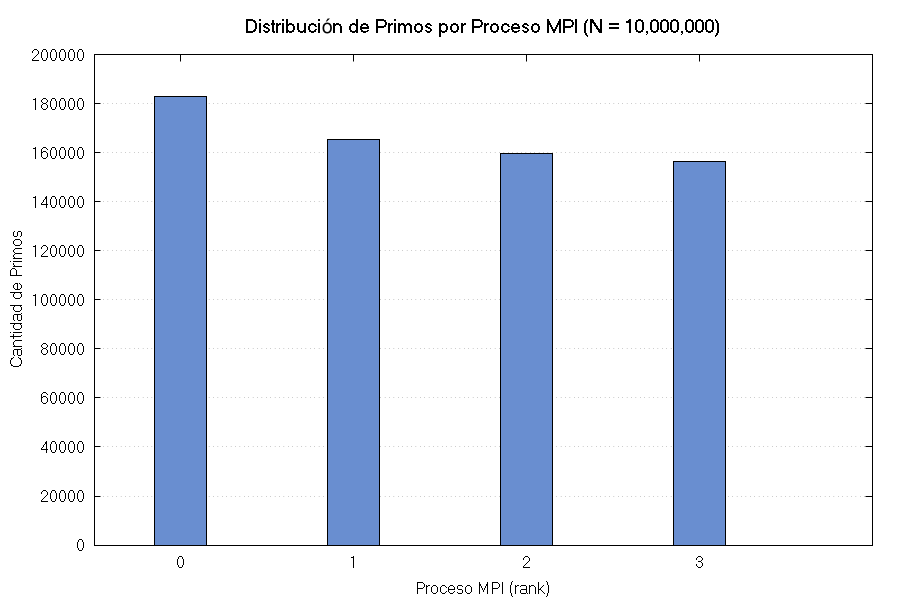
\includegraphics[width=\columnwidth]{distribucion.png}
  \caption{Primos encontrados por cada proceso MPI (4 procesos, $N=10^7$).}
  \label{fig:distribucion}
\end{figure}

\subsection{Curva de speedup}

La Fig.~\ref{fig:speedup} compara el speedup real obtenido con el speedup
ideal $S(p) = p$. El speedup real es sublineal debido a:

\begin{itemize}
  \item La fracción secuencial del programa (cálculo de primos base en
        rank 0 y escritura de archivo), regida por la ley de Amdahl.
  \item La latencia de \texttt{MPI\_Bcast} y \texttt{MPI\_Gather}, que
        crece con el número de procesos.
  \item El overhead del sistema operativo al lanzar procesos MPI en una
        sola máquina compartiendo memoria física.
\end{itemize}

\begin{figure}[h]
  \centering
  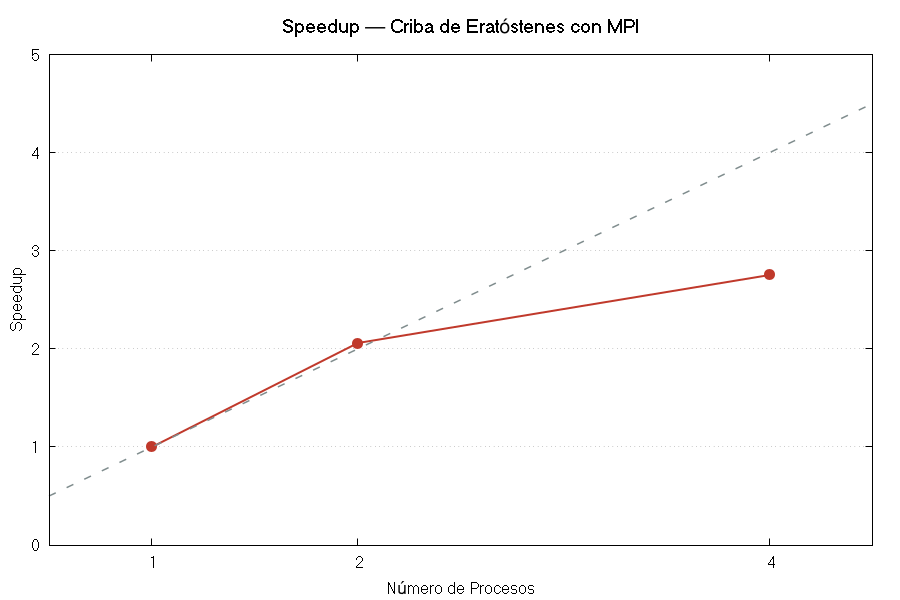
\includegraphics[width=\columnwidth]{speedup.png}
  \caption{Speedup real vs.\ ideal para la criba distribuida.}
  \label{fig:speedup}
\end{figure}

% =============================================================
\section{Conclusiones}

Se implementó exitosamente la Criba de Eratóstenes distribuida utilizando
MPI, obteniendo el resultado correcto de $\pi(10^7) = 664{,}579$ primos en
todos los experimentos.

El speedup alcanzado es cercano al lineal para 2 y 4 procesos, lo que
indica que la fracción paralelizable del algoritmo es dominante. Las
principales limitaciones provienen de la porción secuencial (criba base) y
del overhead de comunicación, ambas moduladas por la ley de Amdahl.

La implementación en un único archivo \texttt{.c} con comentarios extensos
demuestra que los patrones fundamentales de MPI —inicialización, difusión
colectiva y recolección— pueden expresarse de forma clara y legible sin
sacrificar correctitud.

Como trabajo futuro se podría explorar:
\begin{itemize}
  \item Aumentar $N$ a $10^9$ o $10^{10}$ para revelar la escalabilidad en
        rangos donde la fracción secuencial se vuelve negligible.
  \item Combinar MPI con OpenMP (modelo híbrido) para explotar múltiples
        núcleos dentro de cada nodo.
  \item Aplicar técnicas de rueda de factorización (\textit{wheel
        factorization})~\cite{pritchard1982} para reducir el trabajo de
        marcado.
\end{itemize}

% =============================================================
\begin{thebibliography}{9}

\bibitem{knuth1997}
D.~E. Knuth,
\textit{The Art of Computer Programming, Vol. 2: Seminumerical Algorithms},
3rd~ed.
Reading, MA: Addison-Wesley, 1997.

\bibitem{gropp1999}
W.~Gropp, E.~Lusk, and A.~Skjellum,
\textit{Using MPI: Portable Parallel Programming with the Message Passing Interface},
2nd~ed.
Cambridge, MA: MIT Press, 1999.

\bibitem{quinn2003}
M.~J. Quinn,
\textit{Parallel Programming in C with MPI and OpenMP}.
New York, NY: McGraw-Hill, 2003.

\bibitem{pacheco2011}
P.~S. Pacheco,
\textit{An Introduction to Parallel Programming}.
Burlington, MA: Morgan Kaufmann, 2011.

\bibitem{mpiforum2021}
Message Passing Interface Forum,
``MPI: A Message-Passing Interface Standard, Version 4.0,''
Jun. 2021.
[Online]. Available: \url{https://www.mpi-forum.org/docs/mpi-4.0/}

\bibitem{bach1996}
E.~Bach and J.~Shallit,
\textit{Algorithmic Number Theory, Vol. 1: Efficient Algorithms}.
Cambridge, MA: MIT Press, 1996.

\bibitem{pritchard1982}
P.~Pritchard,
``Explaining the wheel factorization,''
\textit{BIT Numerical Mathematics}, vol. 22, no. 4, pp. 442--454, 1982.

\end{thebibliography}

\end{document}
